\section{Implementácia}
\label{chapter:implementacia}

Implementácia aplikácie pre Zepp OS sa zamerala na
použitie senzorov zabudovaných v~hodinkách Amazfit.
Konkrétne sme pracovali s~akcelerometrom a~gyroskopom
na ovládanie pomocou gest zápästia. Naším cieľom bolo
vytvoriť funkčnú aplikáciu, ktorá by umožňovala
intuitívne ovládanie bez nutnosti dotyku displeja.

Vývoj sme začali analýzou údajov z~akcelerometra,
ktorý nám umožnil rozpoznávať základné polohy ruky --
napríklad zdvihnutie ruky nad hlavu alebo presunutie
za chrbát. Pre detekciu rýchlych rotačných pohybov
zápästia, ktoré sú charakteristické pre flickovacie
gestá, sme následne pridali aj spracovanie údajov
z~gyroskopu. Pri vývoji časti bežiacej na hodinkách
sme použili knižnicu \texttt{@zos/sensor} a~Zepp OS
\Gls{api} vo verzii 4.2.

\subsection{Aplikácia na zber dát}
\label{sec:zber-app}

\subsubsection{Architektúra a~rozhranie zberu dát}
Na úvod sme vytvorili skúšobnú aplikáciu pre Zepp OS,
ktorej hlavným cieľom bolo overiť možnosť extrakcie
dát zo senzorov hodiniek Amazfit T-Rex 3. Aplikácia
má tri časti, ktoré sú v~súlade s~architektúrou
Zepp OS Mini Programov: Device App (časť bežiaca na
hodinkách), Side Service (služba bežiaca v~telefóne)
a~Settings App (nastavenia v~Zepp aplikácii).

V~časti Device App sme implementovali zber údajov
z~akcelerometra a~gyroskopu. Tieto dáta sme
v~reálnom čase odosielali do časti Side Service bežiacej
v~telefóne. Keďže Zepp OS natívne nepodporuje priamy
export dát do telefónu, museli sme nájsť alternatívne
riešenie prenosu. Na začiatku sme posielali dáta do
cloudového úložiska Firebase. To nám umožnilo dáta
sťahovať a~spracovávať. Toto riešenie sa však ukázalo
ako nepraktické z~dlhodobého hľadiska. Závislosť na
internetovom pripojení a~oneskorenie pri prenose
znemožnili prácu v~reálnom čase.

Pri hľadaní alternatívy sme zistili, že Side Service
dokáže odosielať dáta aj na lokálny server bežiaci
v~tom istom telefóne. Na základe tohto zistenia sme
sa rozhodli vytvoriť samostatnú Android aplikáciu.
Po spustení vytvorí lokálny \Gls{http} server, ktorý
prijíma spojenie na porte 8080. Dáta zo senzorov sa tak
prenášajú z~hodiniek cez Side Service priamo do Android
aplikácie bez potreby cloudového úložiska.

V~rámci Android aplikácie sme implementovali
rozhranie, ktoré v~reálnom čase zobrazuje
grafy hodnôt akcelerometra a~gyroskopu. Po ukončení
meracej relácie sa všetky nazbierané dáta automaticky
exportujú do \Gls{csv} súboru. Tento súbor následne
slúži na vizualizáciu grafov a~definovanie hraničných
hodnôt pre jednotlivé gestá popísané
v~kapitole~\ref{chapter:gesta}.

Na obrázku~\ref{fig:zber-data-app} je zobrazené
rozhranie aplikácie na zber dát. V~hornej časti sa
nachádza graf gyroskopických dát (osi $g_x$, $g_y$,
$g_z$) a~pod ním graf akcelerometrických dát (osi
$a_x$, $a_y$, $a_z$) za posledných 20 sekúnd.
V~grafe akcelerometra sú farebnými pásmami vyznačené
hraničné hodnoty pre aktuálne zvolené gesto. Výber
gesta je možné zmeniť prostredníctvom rozbaľovacieho
menu nad grafom -- na ľavom snímku je zvolené gesto
\uv{Rise arm}, na pravom \uv{Hand down}.
V~spodnej časti obrazovky sa nachádzajú tlačidlá na
spustenie a~zastavenie lokálneho \Gls{http} servera.
Ukončenie servera zároveň spustí export všetkých
nazbieraných dát do \Gls{csv} súboru pre vizualizáciu
a~spracovanie v~Python skripte.

\begin{figure}[H]
  \centering
  \begin{subfigure}[b]{0.45\textwidth}
    \centering
    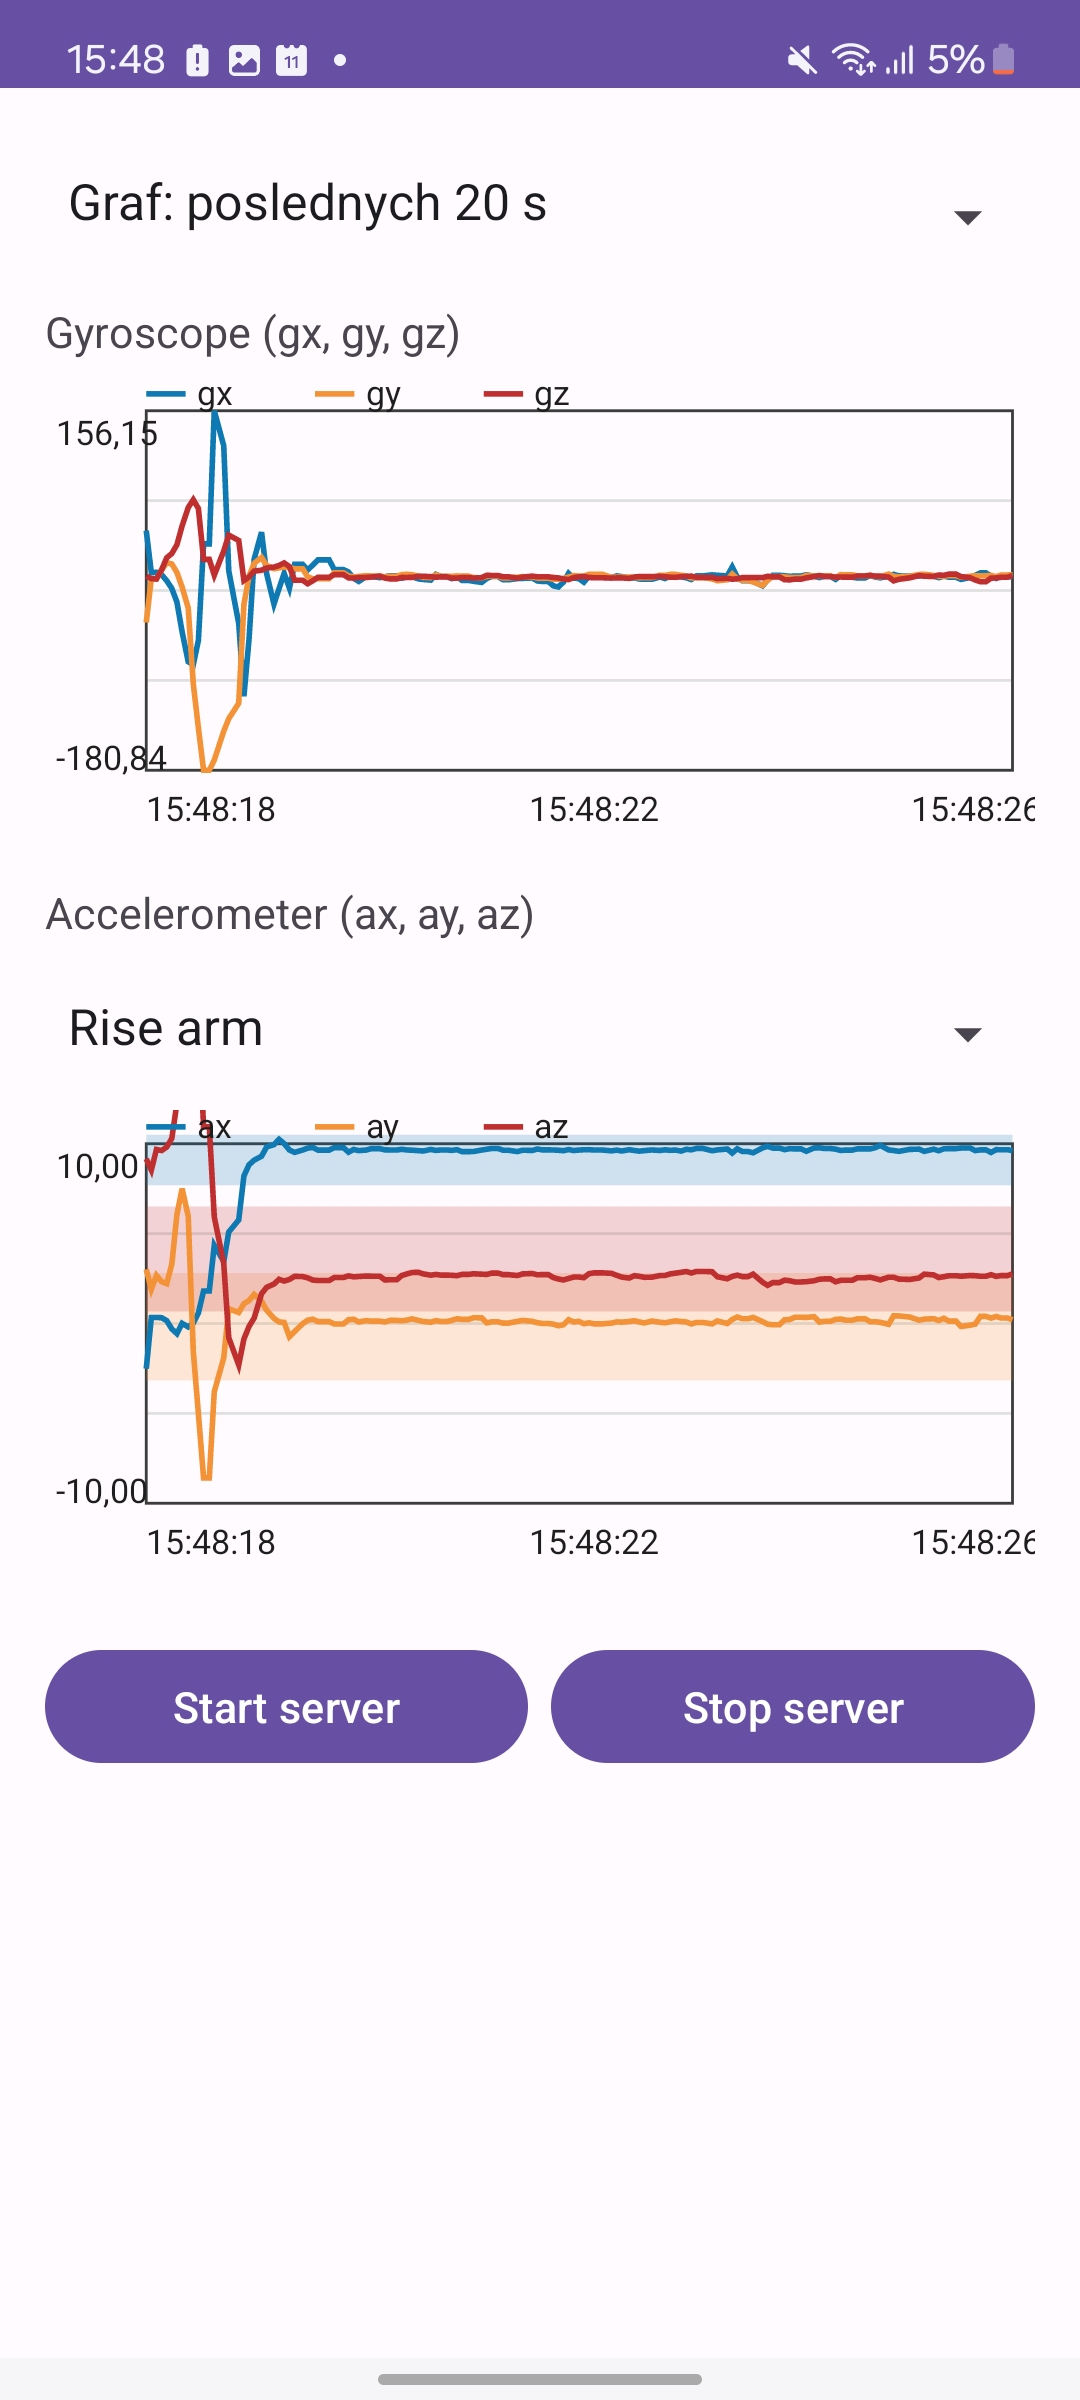
\includegraphics[width=\textwidth]{img/Skusobna-aplikacia1.jpg}
    \caption{Gesto \uv{Rise arm}}
  \end{subfigure}
  \hfill
  \begin{subfigure}[b]{0.45\textwidth}
    \centering
    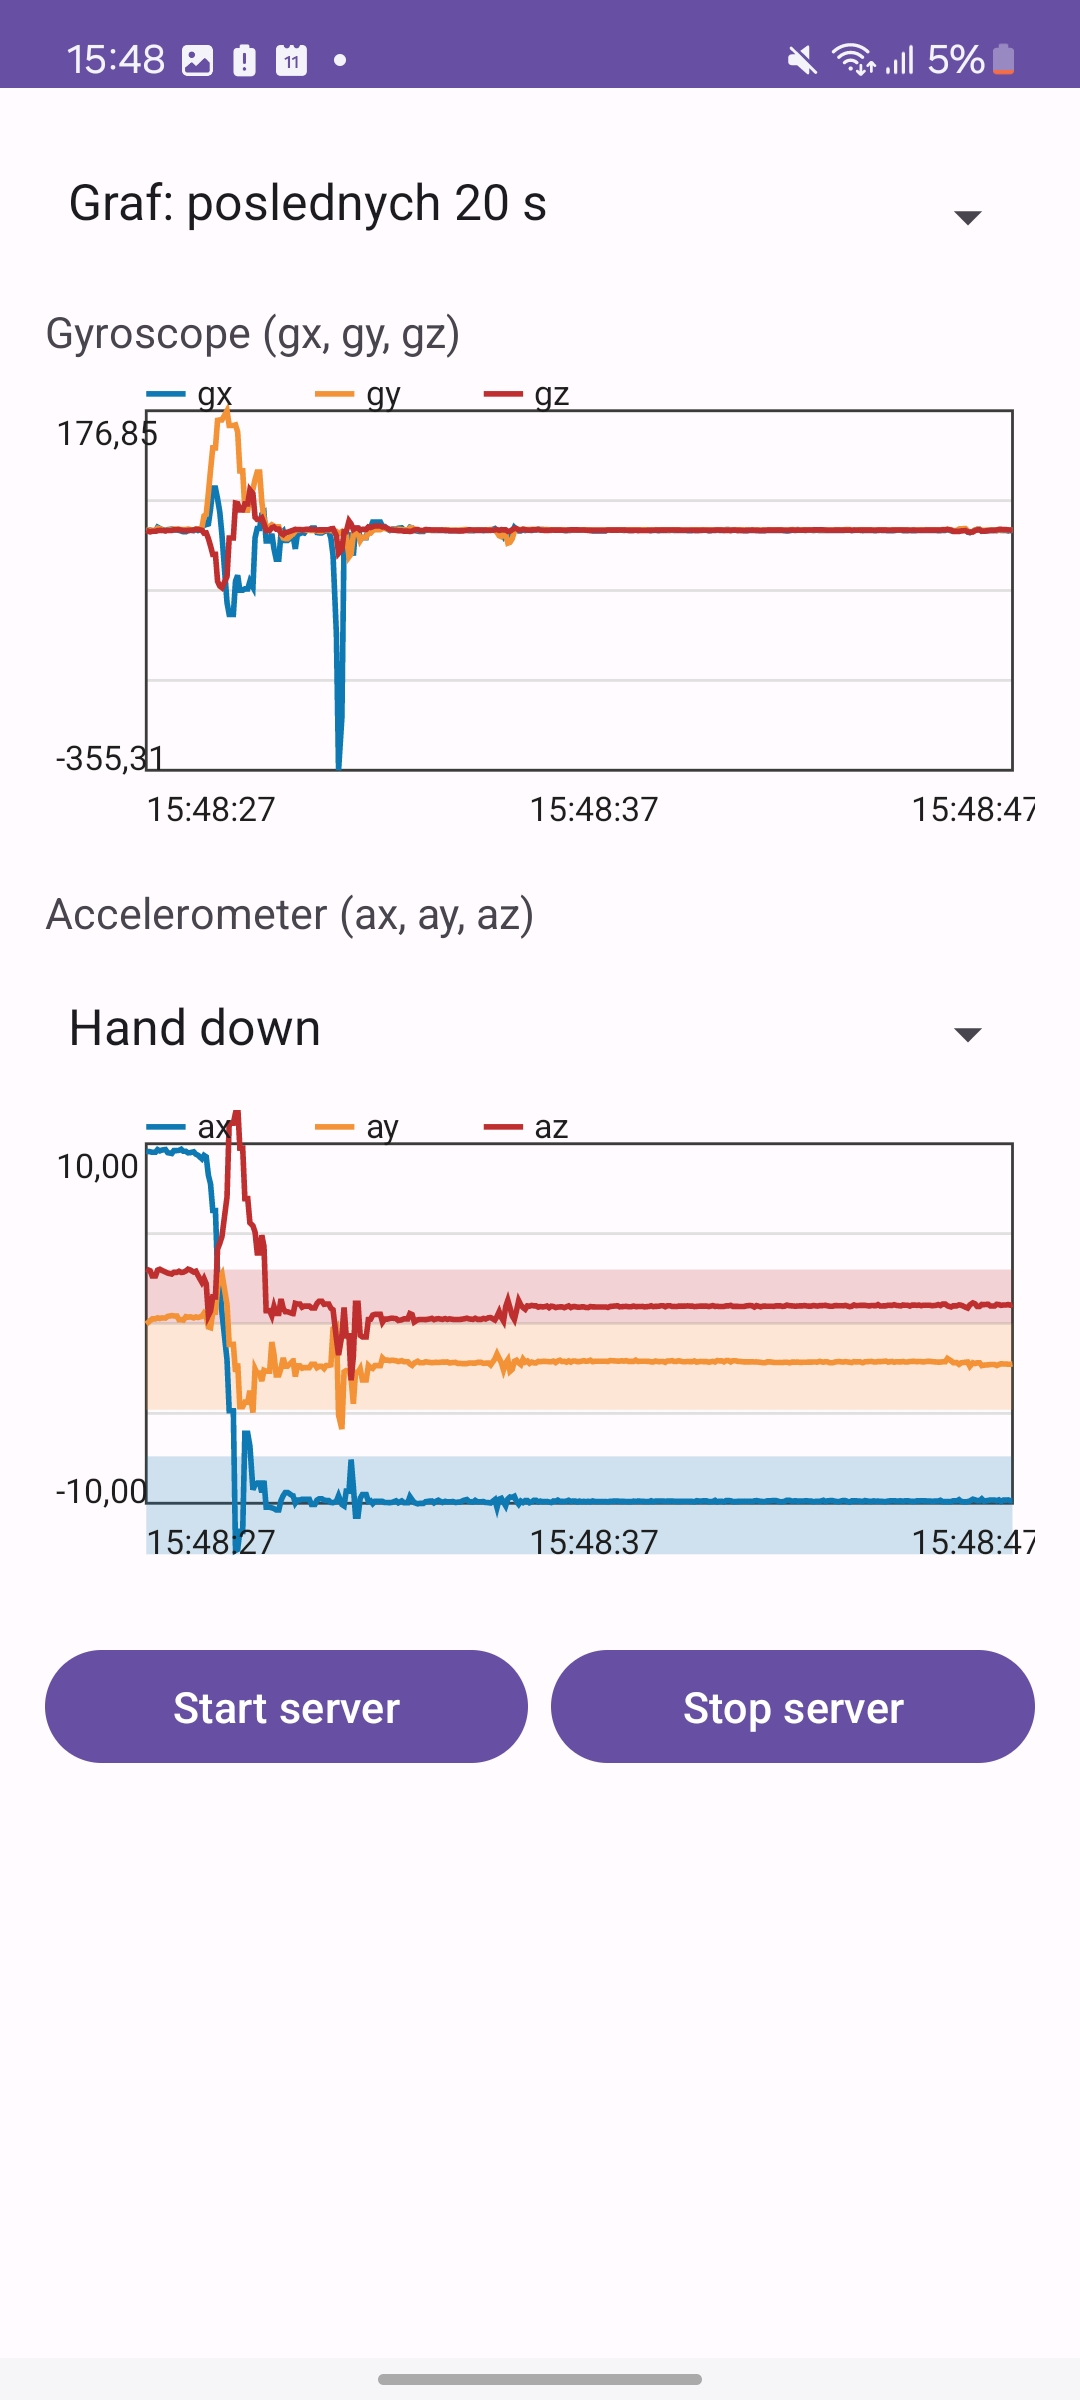
\includegraphics[width=\textwidth]{img/Skusobna aplikacia2.jpg}
    \caption{Gesto \uv{Hand down}}
  \end{subfigure}
  \caption{Rozhranie Android aplikácie na zber dát.}
  \label{fig:zber-data-app}
\end{figure}

\subsubsection{Zber dát}
\label{sec:zber-dát}
Dáta na definovanie hraničných hodnôt sme zbierali
pomocou aplikácie popísanej vyššie. Meranie prebiehalo
v~stoji -- pre každé gesto sme ruku uviedli do
požadovanej polohy a~následne s~ňou pohybovali
v~rámci tejto polohy. Cieľom bolo zachytiť
prirodzenú variabilitu, keďže rozhodca nikdy
nedá ruku do presne rovnakej pozície. Hraničné
hodnoty preto musia obsahovať dostatočnú
toleranciu, ktorá zohľadňuje nielen odchýlky
v~polohe ruky, ale aj skutočnosť, že sa rozhodca
počas zápasu môže nachádzať v~pohybe.

Pre každé gesto sme vykonali 10 meraní. Exportované
\Gls{csv} súbory sme následne spracovali v~Python
nástroji popísanom v~sekcii~\ref{sec:python-skript},
kde sme vizuálne posúdili priebehy senzorových dát
a~na ich základe určili hraničné hodnoty pre
jednotlivé gestá.

\subsection{Python skript na spracovanie a~vizualizáciu dát}
\label{sec:python-skript}
Na definovanie hraničných hodnôt pre jednotlivé gestá
sme vytvorili pomocný nástroj v~jazyku Python, ktorý
slúži ako lokálny webový editor gest. Nástroj je
implementovaný ako \Gls{http} server s užívateľským rozhraním,
ktoré umožňuje načítanie dát z~CSV súboru a~ich vizualizáciu v~grafoch.

Nástroj načíta \Gls{csv} súbory s~nameranými dátami
zo senzorov a~zobrazí ich v~interaktívnych grafoch.
Používateľ si vyberie konkrétne gesto a~\Gls{csv}
súbor, na základe grafu vizuálne posúdi priebeh
senzorových dát a~upraví hraničné hodnoty osí
akcelerometra ($a_x$, $a_y$, $a_z$) alebo prahovú
hodnotu gyroskopu ($g_x$). Nástroj zároveň umožňuje
orezanie \Gls{csv} súborov tak, že používateľ vyberie
relevantný časový úsek a~následne vie uložiť tento segment
do samostatného súboru.

Po uložení hraničných hodnôt nástroj automaticky
vygeneruje Kotlin kód v~tvare \texttt{GestureDefinition},
pripravený na priame vloženie do konfigurácie
Android aplikácie. Príklad vygenerovaného kódu je
uvedený vo výpise kódu~\ref{lst:gesture-definition}.

\begin{lstlisting}[
    style=code-listing,
    language=Kotlin,
    caption={Príklad vygenerovanej definície gesta
    v~jazyku Kotlin},
    label={lst:gesture-definition}
]
GestureDefinition(
    name = "Rise arm",
    message = "Gesture detected: rise arm",
    bands = AccelBands(
        axMin = 1.0,
        axMax = 2.0,
        ayMin = 3.0,
        ayMax = 4.0,
        azMin = 5.0,
        azMax = 6.0
    )
),
\end{lstlisting}

Na obrázku~\ref{fig:gesture-editor} je zobrazené webové rozhranie nástroja na editáciu gest. V~ľavej
časti sa nachádza panel s~výberom \Gls{csv} súboru
a~gesta prostredníctvom rozbaľovacích menu, uloženie
a~orezanie \Gls{csv} súboru, a~vstupné polia pre
manuálnu úpravu hraničných hodnôt jednotlivých osí
akcelerometra. V~pravej časti sú zobrazené 2 interaktívne
grafy, konkrétne horný pre gyroskop a~spodný pre akcelerometer.
V~grafe akcelerometra sú farebnými pásmami
a~prerušovanými čiarami vyznačené aktuálne hraničné
hodnoty pre zvolené gesto. Hranice je možné upraviť
aj priamo v~grafe potiahnutím farebných bodov na
koncoch prerušovaných čiar.

\begin{figure}[H]
  \centering
  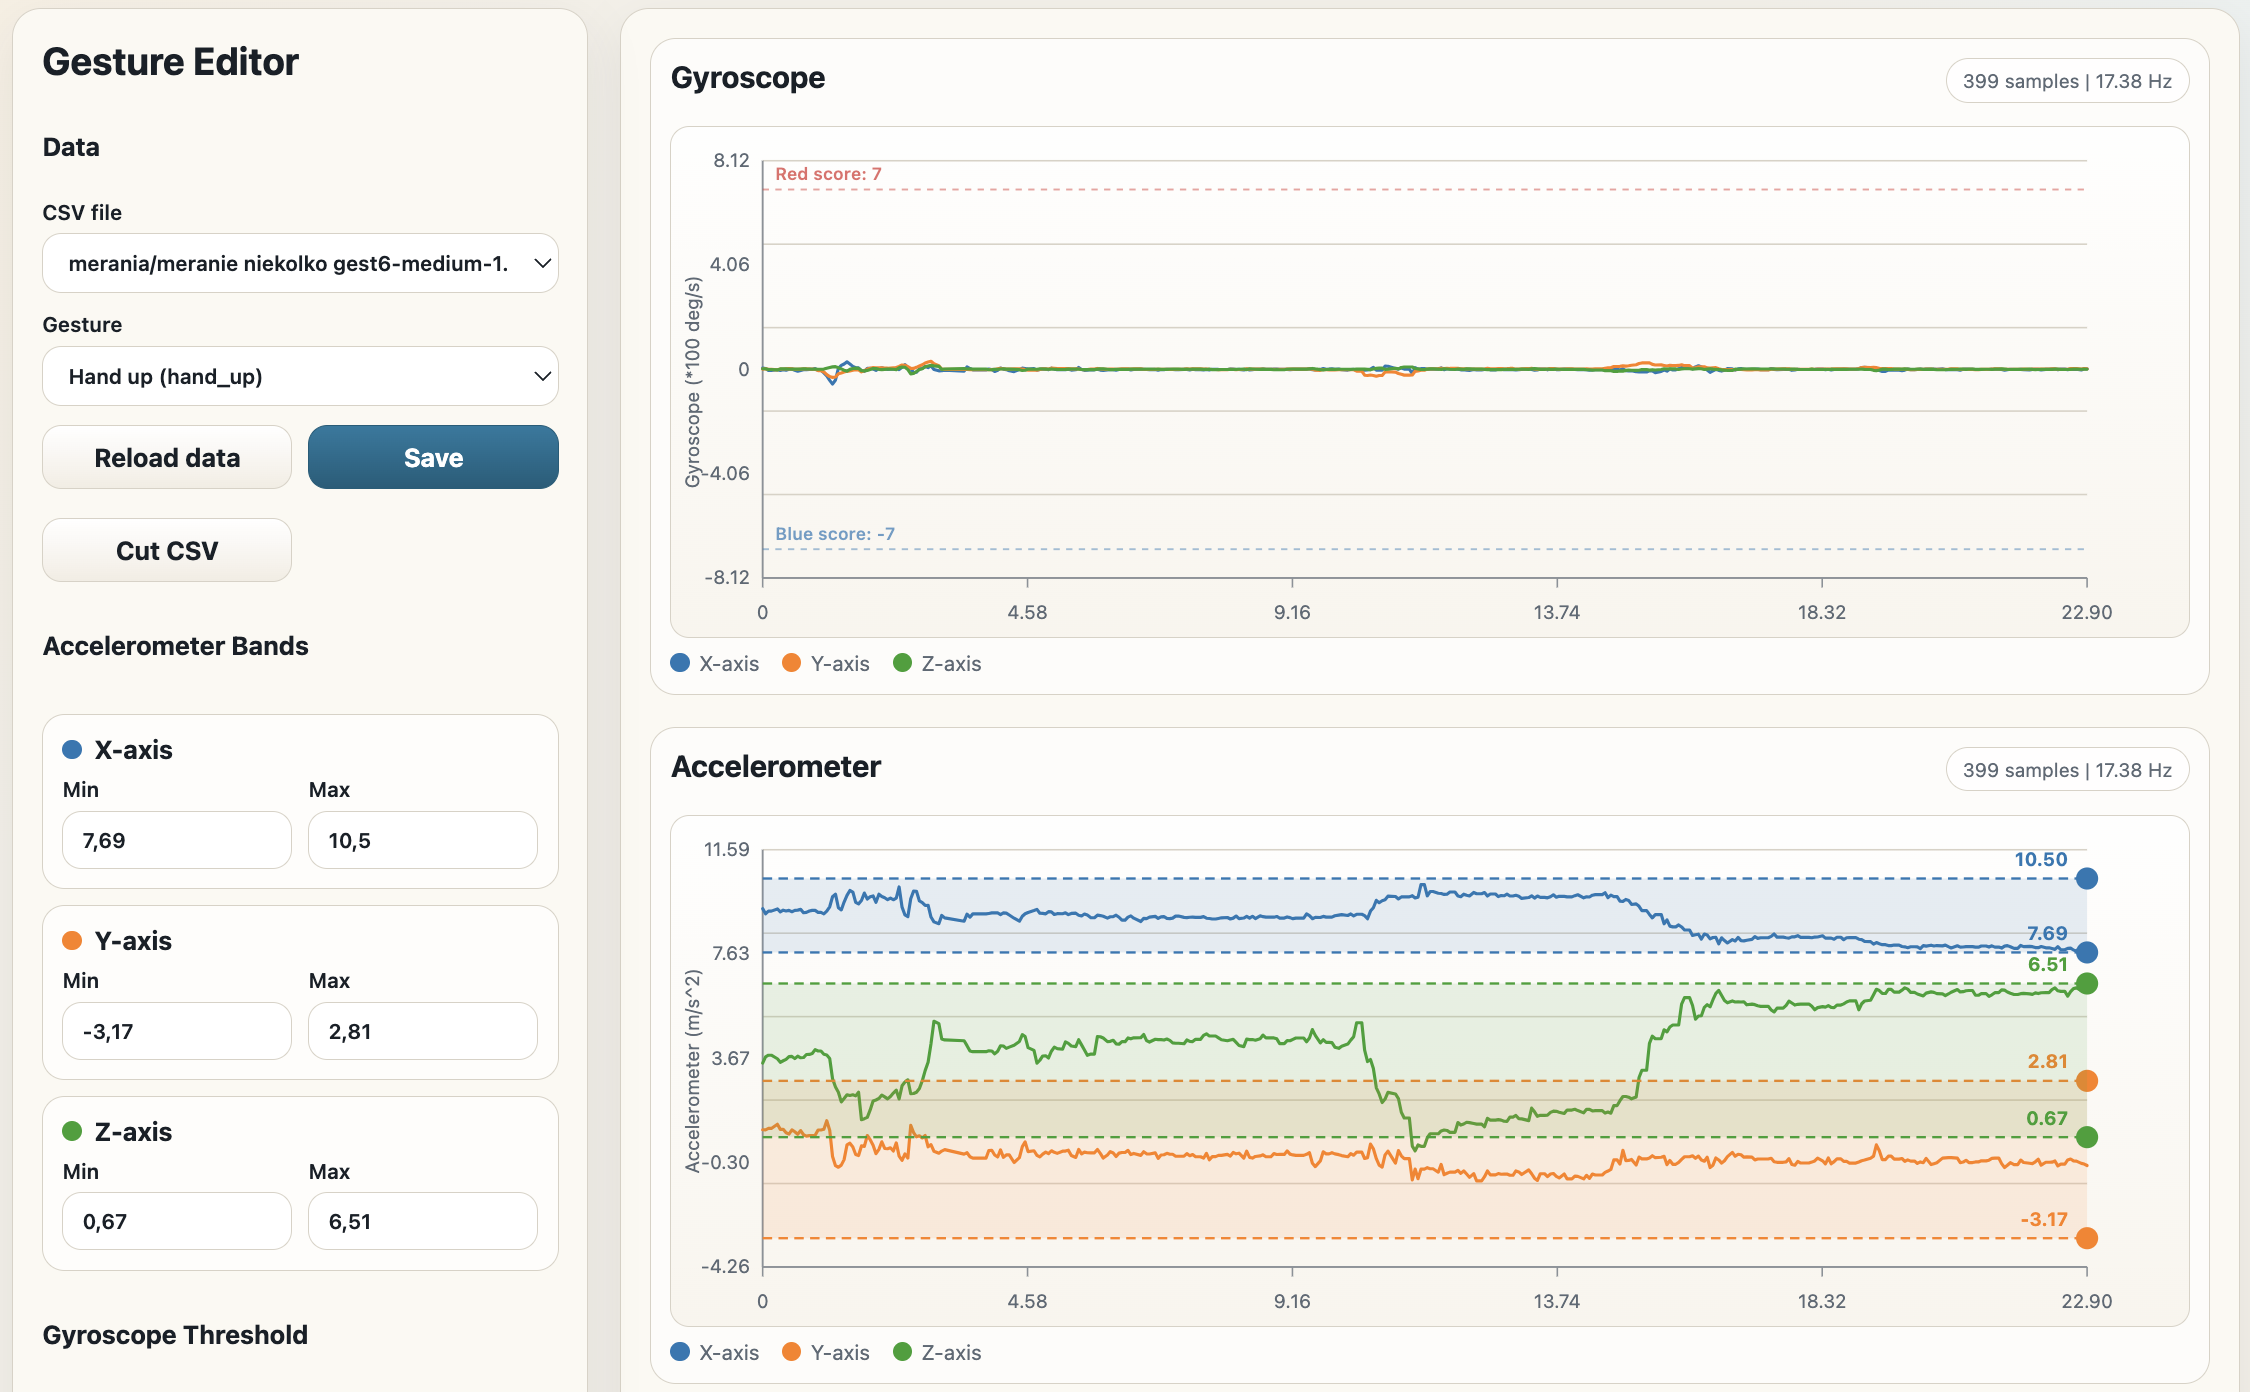
\includegraphics[width=\textwidth]{img/python-script-ukazka.png}
  \caption{Webové rozhranie nástroja na editáciu
    gest}
  \label{fig:gesture-editor}
\end{figure}

\subsection{Aplikácia pre rozpoznávanie gest}
\label{subsec:rozpoznavacia-app}

Finálna aplikácia na rozpoznávanie gest vychádza
zo skúseností získaných pri vývoji aplikácie na zber
dát a~používa rovnakú architektúru (viď
podsekciu~\ref{sec:zber-app}). Hlavným rozdielom je
spôsob spracovania dát -- namiesto exportu do
\Gls{csv} súboru sa údaje vyhodnocujú v~reálnom
čase, výsledné rozpoznané gesto sa spätne odosiela
na hodinky a~slúži na aktualizáciu skóre zápasu.

Celková architektúra systému je znázornená na
obrázku~\ref{fig:architektura}.

\begin{figure}[H]
  \centering
  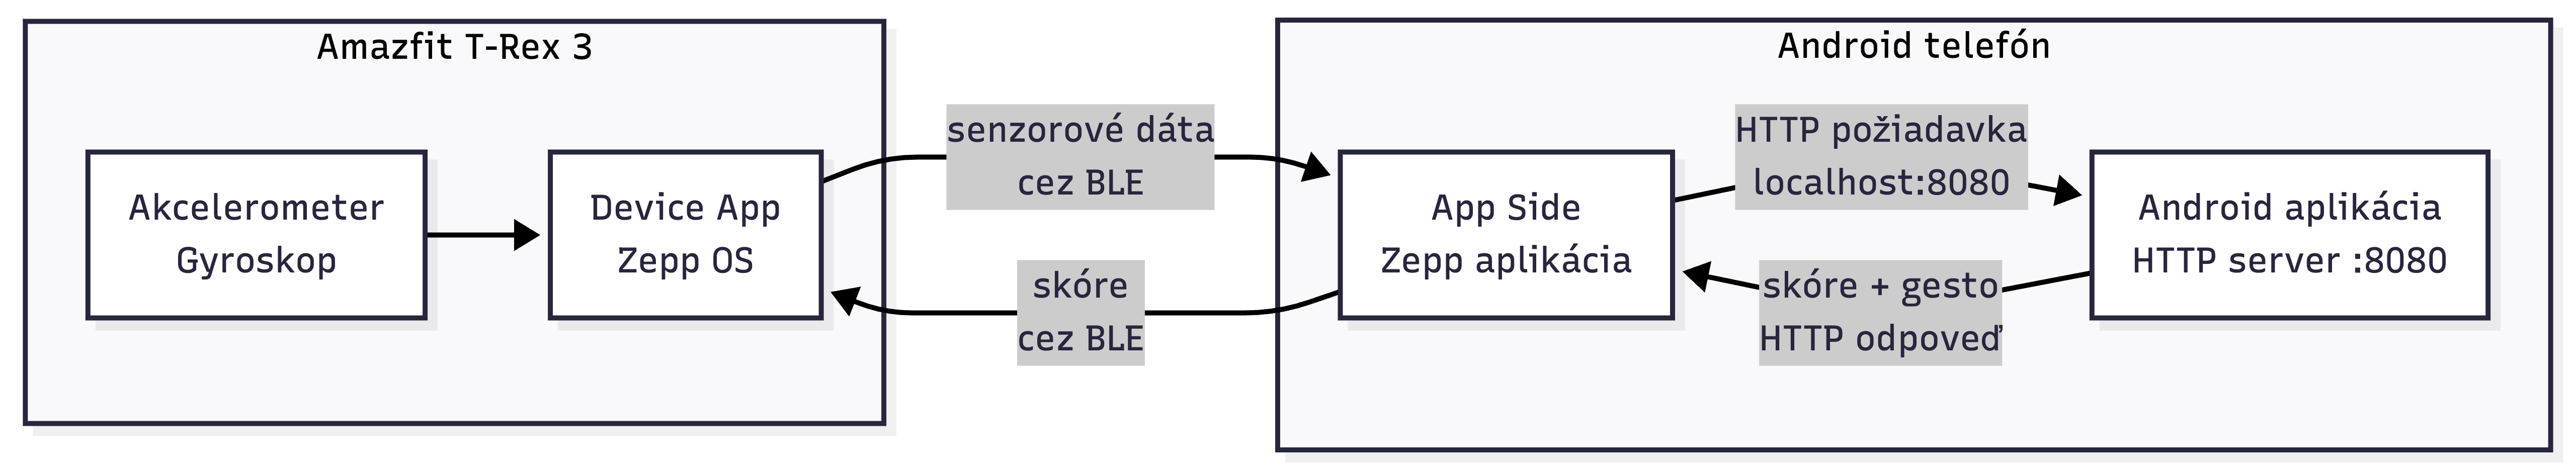
\includegraphics[width=\textwidth]{img/diagrams/flowchart-aplikacia.png}
  \caption{Architektúra systému}
  \label{fig:architektura}
\end{figure}

\subsubsection{Režimy aplikácie}
\label{subsubsec:rezimy-aplikacie}

Aplikácia pracuje v~piatich režimoch, ktoré sú
definované enumeráciou \texttt{GestureMode}:

\begin{itemize}
  \item \textbf{WAITING} -- východiskový režim,
        v~ktorom aplikácia čaká na detekciu gesta.
        Flickovacie gestá (viď podsekciu~\ref{subsubsec:flick})
        sú v~tomto režime ignorované.
  \item \textbf{GESTURE\_RED} -- režim bodovania
        červeného zápasníka. Aplikácia sa do neho
        prepne po detekcii gesta \uv{Rise Arm}
        (viď podsekciu~\ref{subsubsec:rise-arm}).
        Všetky flickovacie gestá zaznamenané počas
        tohto režimu pripočítavajú body červenému
        zápasníkovi.
  \item \textbf{GESTURE\_BLUE} -- režim bodovania
        modrého zápasníka. Aplikácia sa do neho
        prepne po detekcii gesta \uv{Hand Back}
        (viď podsekciu~\ref{subsubsec:hand-back}).
        Všetky flickovacie gestá zaznamenané počas
        tohto režimu pripočítavajú body modrému
        zápasníkovi.
  \item \textbf{WARNING\_RED} -- režim napomenutia
        červeného zápasníka. Aplikácia sa do neho prepne
        po detekcii gesta \uv{NAPOMENUTIE -- červený}.
        Bodovanie je obmedzené na modrého zápasníka --
        všetky flicky pripočítavajú body modrému zápasníkovi.
  \item \textbf{WARNING\_BLUE} -- režim napomenutia
        modrého zápasníka. Analogicky k~predchádzajúcemu,
        všetky flicky sa pripočítavajú výhradne červenému
        zápasníkovi.
\end{itemize}

Režimy \texttt{GESTURE\_RED}, \texttt{GESTURE\_BLUE},
\texttt{WARNING\_RED} a~\texttt{WARNING\_BLUE} zdieľajú
spoločnú vlastnosť -- vo všetkých štyroch sa vyhodnocujú
flickovacie gestá. O~tom, ktorému zápasníkovi sa
zaznamenaný flick pripočíta, rozhoduje výhradne aktuálny
režim aplikácie, nie smer ani charakter samotného flicku.
Návrat do režimu \texttt{WAITING} sa vo všetkých
prípadoch vykoná gestom \uv{Hand Down}.

\subsubsection{Debug mód}
\label{app:debug-final}
Debug mód Android aplikácie slúži na monitorovanie
a~ladenie rozpoznávania gest v~reálnom čase. Oproti
pôvodnej aplikácii na zber dát bolo rozhranie
rozšírené o~zobrazenie aktuálne rozpoznaného gesta,
režimu aplikácie a~priebežného skóre. Po spustení sa
predvolene zobrazuje grafové zobrazenie senzorových
dát, ktoré umožňuje vizuálne sledovať priebeh
detekcie gest.

V~debug móde sa do logu zaznamenávajú aj pomocné
aktivačné gestá \uv{Rise Arm} a~\uv{Hand Back},
ktorým je zároveň priradená vibračná odozva
(viď podsekciu~\ref{subsubsec:vibracna-odozva}).
Aplikácia v~tomto móde implementuje aj 30-sekundový
časomer pasivity -- po detekcii gesta pasivity sa
spustí odpočet a~v~prípade jeho uplynutia bez
zaznamenaného bodovania sa súperovi pasívneho
zápasníka automaticky pridelí trestný bod.

Na obrázku~\ref{fig:debug-scoring} je zobrazený
stav aplikácie počas sekvencie bodovania pre
červeného zápasníka. V~hornej časti obrazovky
vidíme aktuálny režim (\texttt{GESTURE\_RED})
a~informáciu o~poslednom rozpoznanom geste
\uv{Rise Arm}. Pod tým je zobrazené priebežné
skóre -- Blue: 0, Red: 2. Na grafe gyroskopu sú
viditeľné výrazné špičkové výkyvy na osi $g_x$,
ktoré zodpovedajú jednotlivým flickovacím gestám.
Každý výkyv prekračujúci nastavený prah pridelil
jeden bod červenému zápasníkovi podľa aktívneho
režimu bodovania v~čase jeho detekcie. V~grafe
akcelerometra sú viditeľné prechody hodnôt
zodpovedajúce aktivačnému gestu \uv{Rise Arm}
(vstup do režimu \texttt{GESTURE\_RED}), po ktorom
nasledovali flickovacie gestá. Farebné pásma
v~pozadí grafu akcelerometra znázorňujú nastavené
prahové intervaly pre rozpoznanie polohy ruky
\uv{Hand up}.

\begin{figure}[H]
  \centering
  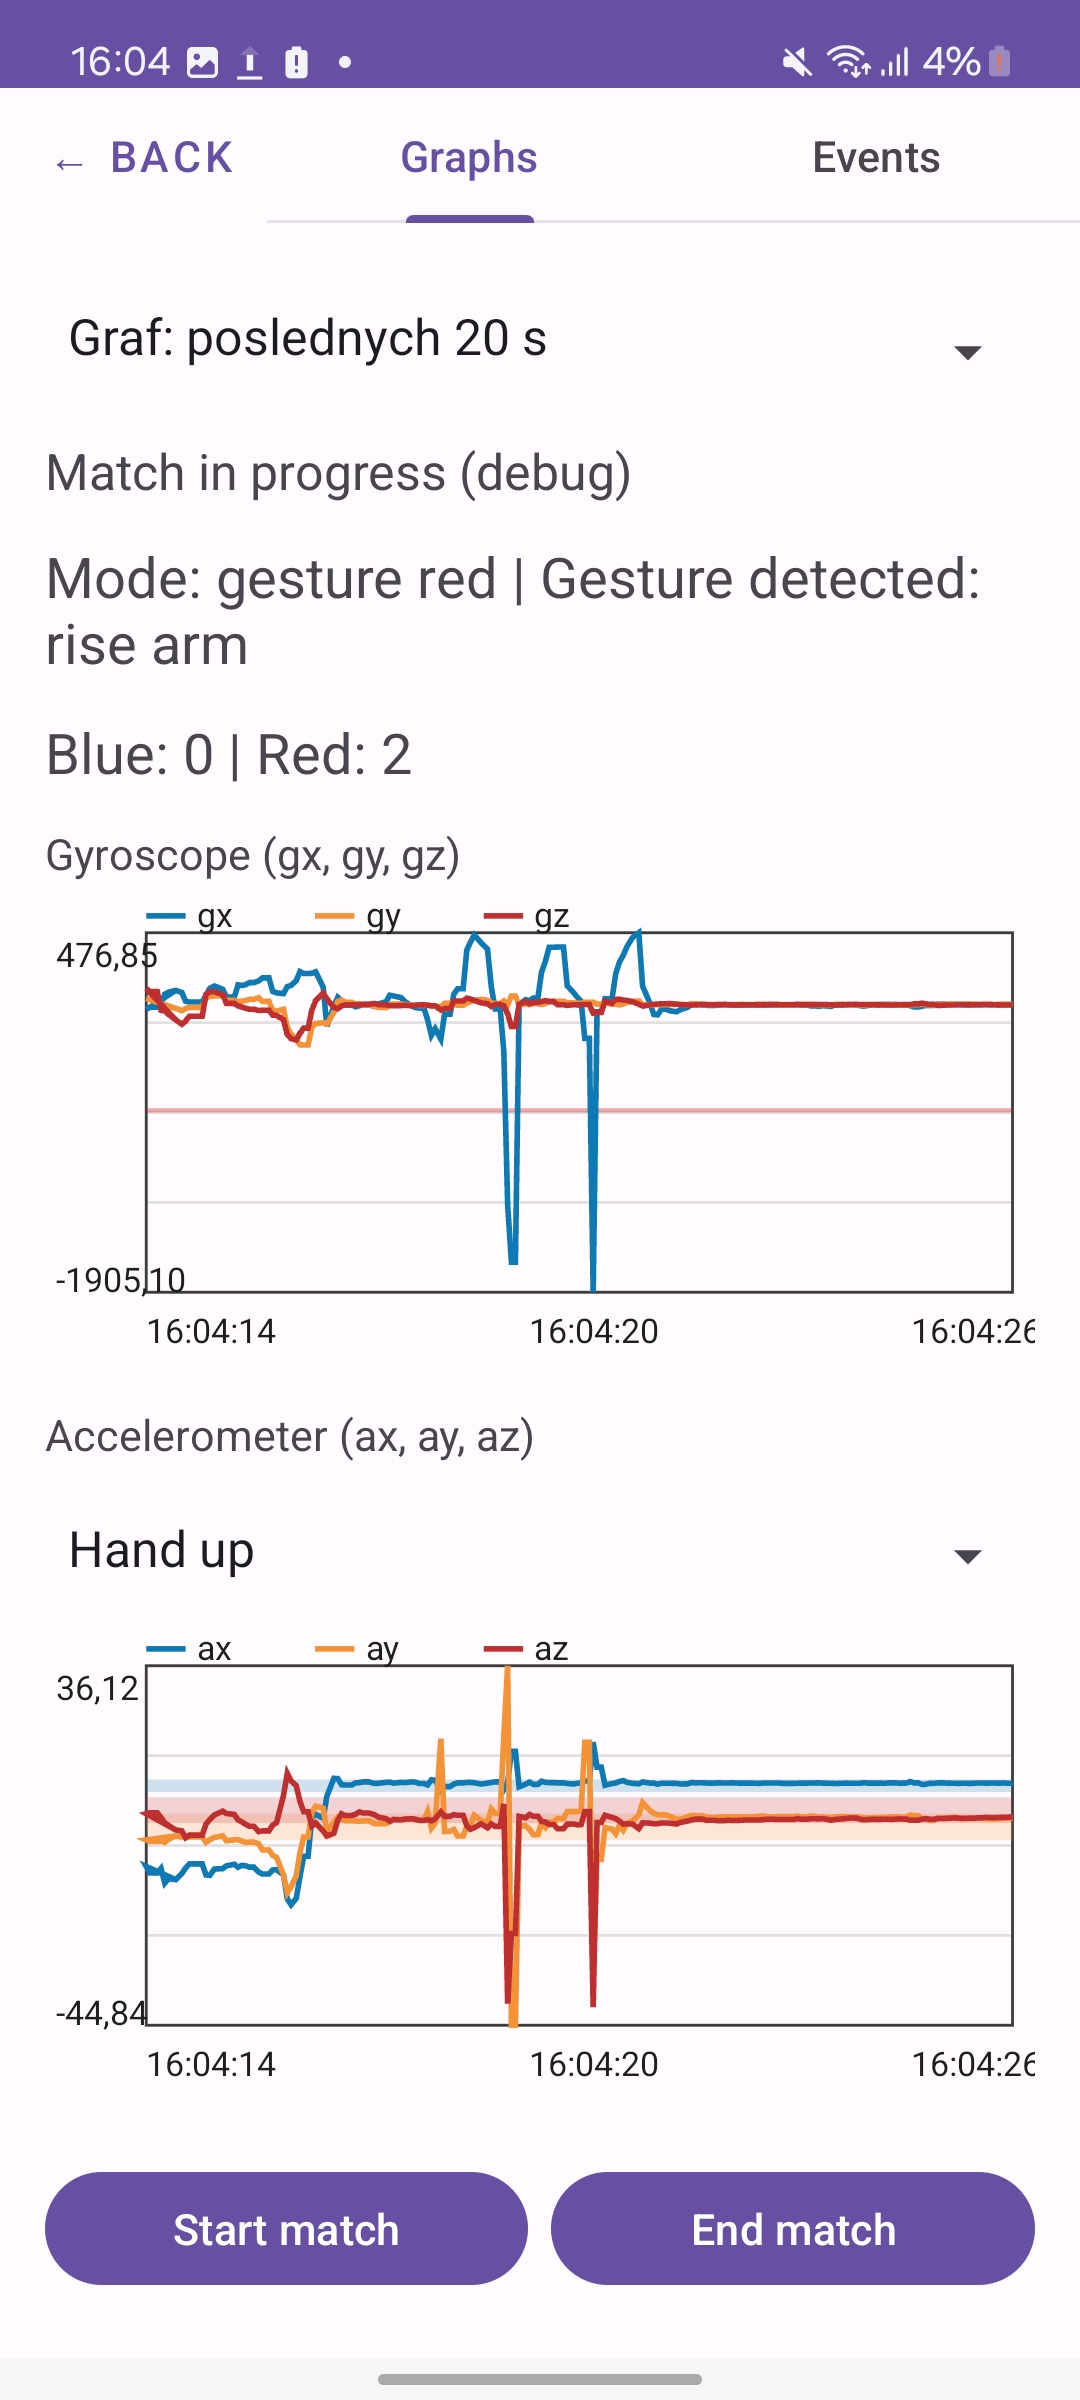
\includegraphics[width=0.35\textwidth]{img/gesto-aplikacia-debug.jpg}
  \caption{Debug mód -- stav počas sekvencie bodovania (Blue: 0, Red: 2)}
  \label{fig:debug-scoring}
\end{figure}

\subsubsection{Produkčný mód}
\label{app:prod-final}

Produkčný mód Android aplikácie je určený pre
reálne použitie počas zápasu. Na rozdiel od debug
módu sa po spustení nezobrazuje grafové zobrazenie
senzorov -- predvolene je aktívna záložka so~záznamom
udalostí. Grafy senzorov zostávajú dostupné
v~samostatnej záložke pre prípad potreby.

V~hornej časti obrazovky je zobrazené priebežné
skóre v~tvare Blue: X | Red: Y. Pod ním sa nachádza
zoznam udalostí, kde je každá udalosť zaznamenaná
s~presnou časovou značkou. Zaznamenávajú sa iba
udalosti relevantné pre priebeh zápasu -- udelenie
bodov, napomenutia a~TOUCHE. Pomocné gestá ako
\uv{Rise Arm} a~\uv{Hand Back} sa do~logu nezapisujú,
keďže slúžia len na aktiváciu režimu bodovania.

Na obrázku~\ref{fig:prod-mode} je zobrazený príklad
produkčného rozhrania po sérii udalostí simulujúcich
reálny priebeh zápasu. V~logu sú viditeľné dva body
pridelené červenému zápasníkovi, následne dva body pre modrého
zápasníka, potom napomenutie červeného zápasníka so~zápisom \uv{Warning
red} a~následné dva trestné body pridelené modrému
zápasníkovi. Sekvenciu uzatvára signalizácia TOUCHE --
lopatkového víťazstva. Konečné skóre simulovaného
zápasu je Blue: 4 | Red: 2.

\begin{figure}[H]
  \centering
  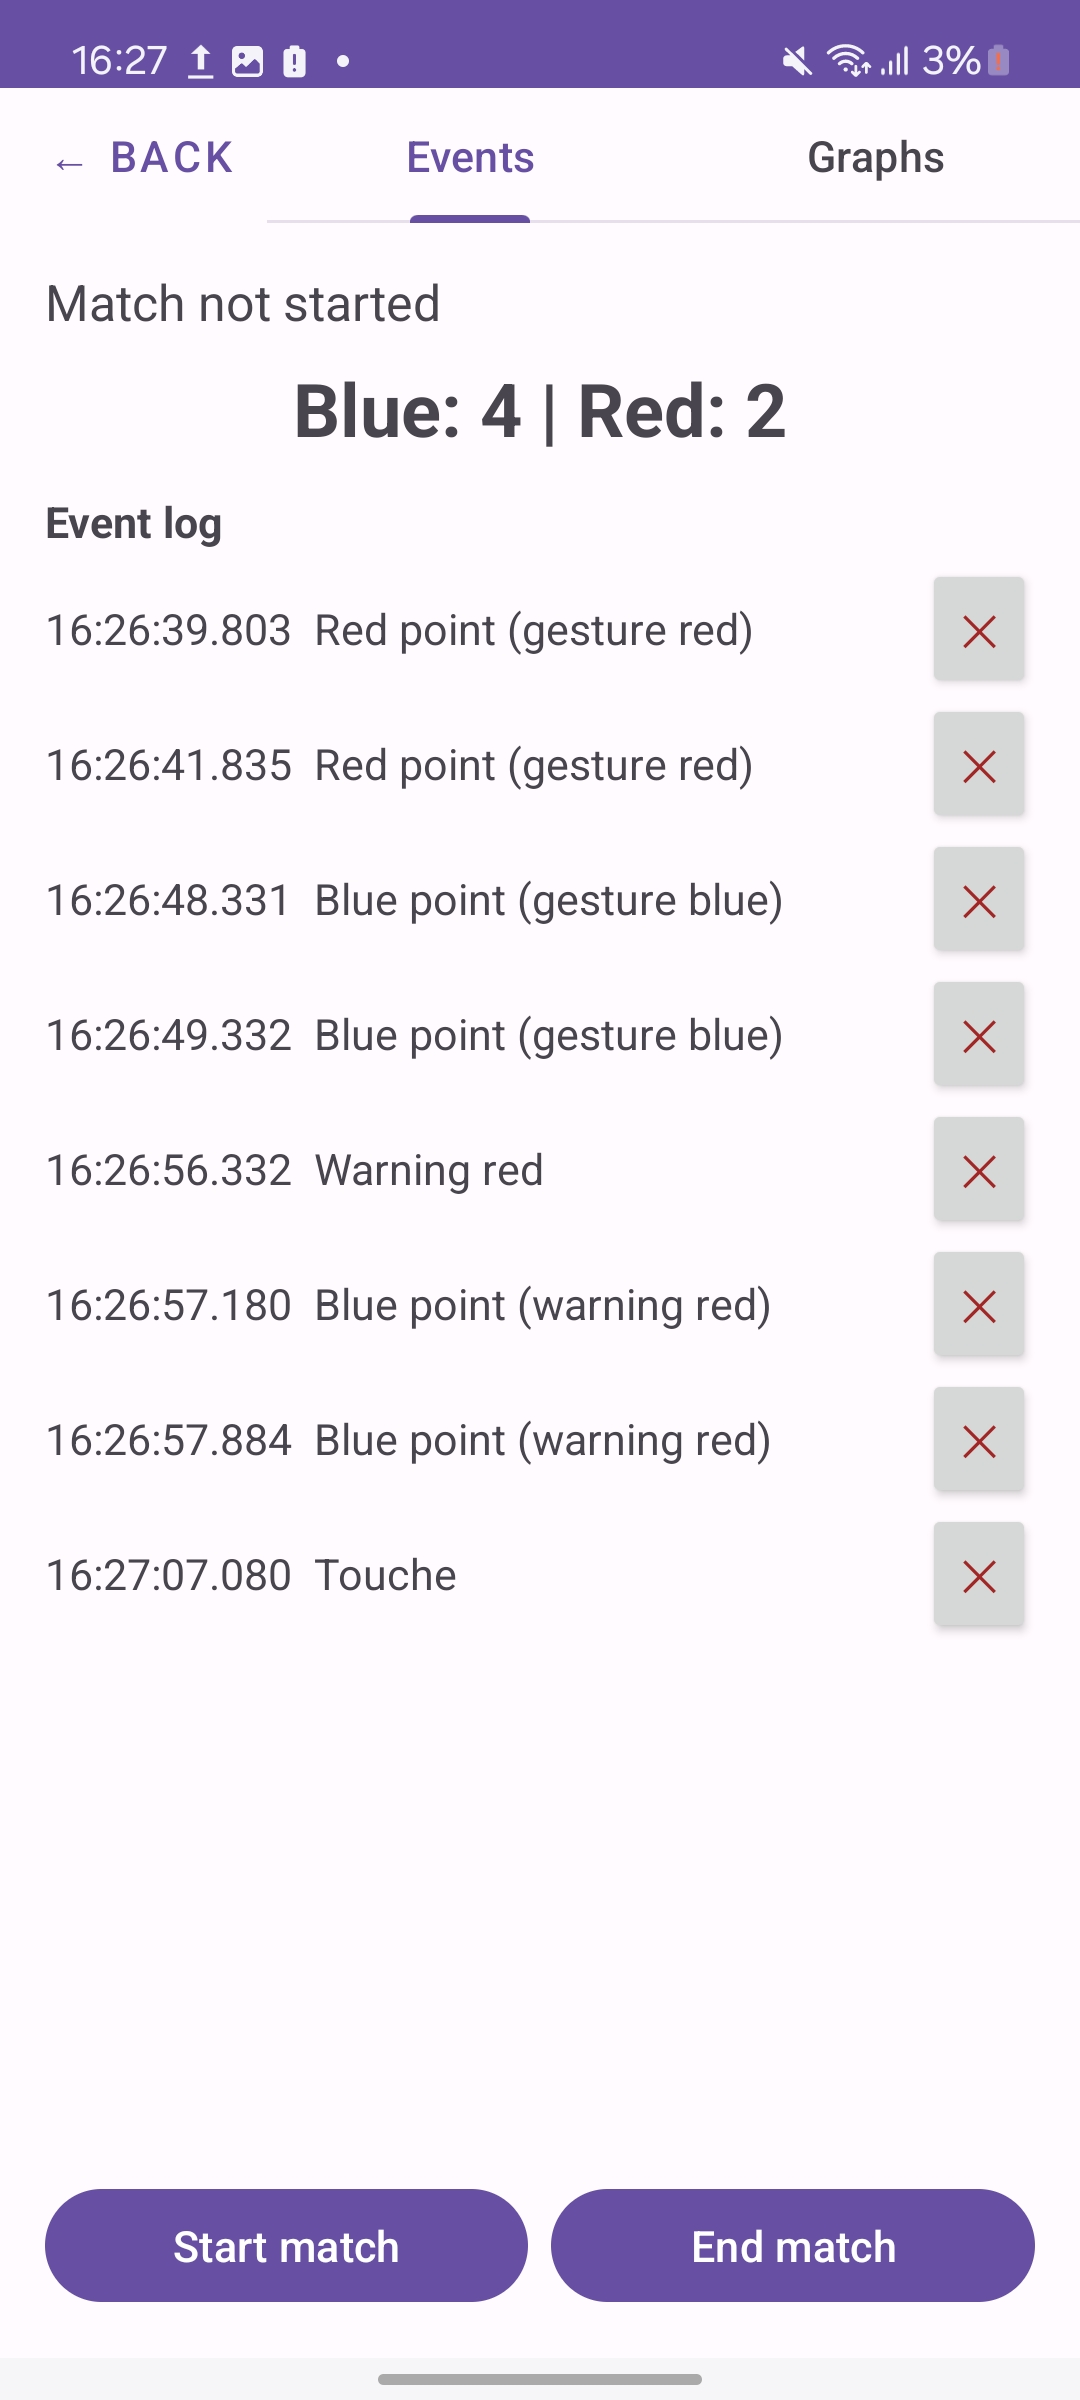
\includegraphics[width=0.4\textwidth]{img/gesto-aplikacia-prod.jpg}
  \caption{Produkčný mód Android aplikácie -- záznam udalostí počas simulovaného zápasu}
  \label{fig:prod-mode}
\end{figure}

\subsubsection{Zhrnutie rozdielov medzi produkčným a~debug módom}
\label{subsubsec:hlavne-rozdiely}

Hlavné rozdiely medzi oboma módmi sú prehľadne zhrnuté
v~tabuľke~\ref{tab:rozdiely-modov}.

\begin{table}[H]
  \centering
  \caption{Porovnanie funkcionality debug a~produkčného módu}
  \label{tab:rozdiely-modov}
  \renewcommand{\arraystretch}{1.4}
  \begin{tabularx}{\textwidth}{
      >{\raggedright\arraybackslash}X
      >{\centering\arraybackslash}p{0.18\textwidth}
      >{\centering\arraybackslash}p{0.18\textwidth}
    }
    \toprule
    \textbf{Funkcia}                                & \textbf{Debug} & \textbf{Produkčný} \\
    \midrule
    Grafové zobrazenie senzorov                     & áno            & áno (vedľajšia záložka)                \\
    \midrule
    Logovanie pomocných gest (Rise Arm, Hand Back)  & áno            & nie                \\
    \midrule
    Vibračná odozva pri pomocných gestách           & áno            & nie                \\
    \midrule
    30-sekundový časomer pasivity                   & áno            & nie                \\
    \midrule
    Automatické pridelenie trestného bodu           & áno            & nie                \\
    \bottomrule
  \end{tabularx}
\end{table}

Hlavným dôvodom obmedzenej funkcionality v~produkčnom móde
je skutočnosť, že podľa zápasníckych pravidiel \Gls{uww}
musí byť udelenie trestného bodu za pasivitu odsúhlasené
bočným rozhodcom a~vedúcim žinenky. Ide o~samostatný
proces validácie, ktorý nie je možné spoľahlivo zachytiť
prostredníctvom hodiniek hlavného rozhodcu. Zároveň
priebeh zápasu môže byť kedykoľvek prerušený (opustenie
žinenky, zranenie či technická prestávka), čo by si
vyžiadalo implementáciu ďalších gest a~funkcionalít
presahujúcich rámec diplomovej práce.

Vibračnú odozvu pri pomocných gestách \uv{Rise Arm}
a~\uv{Hand Back} sme v~produkčnom móde vypli preto, že
tieto gestá sa počas zápasu vykonávajú pri každom
bodovaní, čo by viedlo k~nadmernému počtu vibračných
impulzov v~krátkom časovom úseku.

\subsubsection{Vibračná odozva}
\label{subsubsec:vibracna-odozva}

Pre zlepšenie používateľského zážitku a~zabezpečenie
spätnej väzby pre rozhodcu sme implementovali
vibračnú odozvu prostredníctvom vibrácií hodiniek.
Každý typ udalosti má priradenú odlišnú vibračnú
schému, ktorá sa líši počtom impulzov a~ich trvaním.
Rozhodca tak aj bez pohľadu na displej vie, aká
udalosť bola zaznamenaná.

V~rámci aplikácie sme definovali tri typy vibračných
impulzov, ktoré slúžia ako základné stavebné jednotky
pre zložené vibračné schémy:

\begin{itemize}
  \item \textbf{Krátky impulz} (\textit{short})
        \label{vib:short} -- vibračný impulz s~trvaním
        250\,ms.

  \item \textbf{Dlhý impulz} (\textit{long})
        \label{vib:long} -- vibračný impulz s~trvaním
        500\,ms. Pri testovaní sa ukázalo, že 500\,ms
        je maximálna dosiahnuteľná dĺžka spojitej
        vibrácie -- firmvér hodiniek motor po tomto
        intervale automaticky zastaví.

  \item \textbf{Silný krátky impulz}
        (\textit{short\_strong}) \label{vib:short-strong}
        -- jednorazový impulz s~trvaním 20\,ms a~vyššou
        intenzitou.
\end{itemize}

\noindent V~aplikácii rozlišujeme šesť typov udalostí, pri ktorých sa
spustí vibračná odozva:

\begin{itemize}
  \item \textbf{Ukončenie bodovania} -- nastáva po vykonaní
        gesta \uv{Hand Down} v~ktoromkoľvek z~bodovacích režimov
        (\texttt{GESTURE\_RED}, \texttt{GESTURE\_BLUE},
        \texttt{WARNING\_RED}, \texttt{WARNING\_BLUE} --
        viď podsekciu~\ref{subsubsec:rezimy-aplikacie}). Počet
        následných krátkych impulzov zodpovedá počtu bodov
        pridelených v~práve ukončenej sekvencii.

  \item \textbf{TOUCHE} -- nastáva po detekcii gesta \uv{TOUCHE}.
        Päť po sebe nasledujúcich krátkych impulzov tvorí
        výraznú schému, ktorú nemožno zameniť so žiadnou inou
        udalosťou.

  \item \textbf{Prechod do režimu napomenutia} -- nastáva po
        detekcii gesta \uv{NAPO\-MENUTIE -- červený} alebo
        \uv{NAPOMENUTIE -- modrý}.

  \item \textbf{Aktivácia režimu bodovania} -- nastáva po
        detekcii aktivačného gesta \uv{Rise Arm} alebo
        \uv{Hand Back} (iba v~debug móde).

  \item \textbf{Pasivita} -- nastáva po
        detekcii gesta \uv{PASIVITA -- červený} alebo
        \uv{PASIVITA -- modrý}.

  \item \textbf{Trestný bod za pasivitu} -- nastáva automaticky
        po uplynutí 30-sekundového odpočtu pasivity bez
        zaznamenaného bodovania (iba v~debug móde, viď
        podsekciu~\ref{app:debug-final}).
\end{itemize}

Mapovanie konkrétnych udalostí na typy vibračných impulzov
je uvedené v~tabuľke~\ref{tab:vibracna-odozva}.

\begin{table}[H]
  \centering
  \caption{Prehľad vibračnej odozvy pri jednotlivých udalostiach}
  \label{tab:vibracna-odozva}
  \renewcommand{\arraystretch}{1.4}
  \begin{tabularx}{\textwidth}{
      >{\raggedright\arraybackslash}p{0.30\textwidth}
      >{\raggedright\arraybackslash}X
      >{\raggedright\arraybackslash}X
      >{\centering\arraybackslash}p{0.13\textwidth}
    }
    \toprule
    \textbf{Udalosť}              & \textbf{Impulz}           & \textbf{Následné impulzy}    & \textbf{Mód}     \\
    \midrule
    Ukončenie bodovania           & 1\,$\times$\,dlhý         & $N$\,$\times$\,krátky $^{*}$ & oba              \\
    \midrule
    TOUCHE                        & 5\,$\times$\,krátky       & --                           & oba              \\
    \midrule
    Prechod do režimu napomenutia & 2\,$\times$\,krátky       & --                           & oba              \\
    \midrule
    Aktivácia režimu bodovania    & 1\,$\times$\,silný krátky & --                           & len \emph{debug} \\
    \midrule
    Pasivita                      & 2\,$\times$\,krátky       & --                           & oba              \\
    \midrule
    Trestný bod za pasivitu       & 1\,$\times$\,dlhý         & --                           & len \emph{debug} \\
    \bottomrule
  \end{tabularx}

  \vspace{0.5em}
  {\footnotesize $^{*}$ $N$ -- počet bodov pridelených v~práve ukončenej bodovacej sekvencii.}
\end{table}